\documentclass[12pt]{article}
\usepackage[utf8]{inputenc}
\usepackage{amsmath}
\usepackage{systeme}
\usepackage{amsfonts}
\usepackage{graphicx}
\usepackage{enumitem}
\usepackage{hyperref}
\usepackage{xcolor}
\usepackage{kbordermatrix}
\usepackage{centernot}
\usepackage{xcolor}

\title{%
	\textbf{Notițe Seminar 2}}

\begin{document}
	
	\maketitle
	
	\textbf{\large{Intro}}:
	\begin{enumerate}
		\item 	Dacă la seminarul trecut am lucrat cu probabilități într-un mod mai \textit{low-level}, începând cu seminarul acesta vom lucra cu ele mai \textit{high-level}:
		
		Se aruncă un zar. Care este probabilitatea să cadă un număr par?
		
		$\Omega = \{1,2,3,4,5,6\}$
		
		Pentru că nu există informații suplimentare, vom presupune că rezultatele sunt echiprobabile.
		
		$P(\text{iese număr par}) = P(\{2,4,6\}) = \frac{1}{2}$
		
		$P(\text{iese număr impar}) = P(\{1,3,5\}) = \frac{1}{2}$
		
		Dacă pe noi în continuare nu ne interesează decât P(iese număr par) și P(iese număr impar), putem uita de $\Omega$ și de cum am calculat cele 2 probabilități. Totodată, dacă vi s-ar fi furnizat deja P(iese număr par) și P(iese număr impar) nu ar mai fi trebuit să spuneți cât e $\Omega$ și să calculați cele 2 probabilități. Astfel, lucrând doar cu P(iese număr par) și P(iese număr impar), putem spune că suntem la un nivel mai \textit{high}.
		
		\item 	Dacă până acum, ne-a interesat dacă un eveniment \textbf{se realizează sau nu} (deci, dacă dorim numeric: 0 - nu s-a realizat și 1 - s-a realizat) - număr par sau nu, nimerește ținta sau nu -, de acum vom putea răspunde și la alte întrebări: \textbf{cât} câștigi dacă iese numărul 1 la aruncarea zarului?, \textbf{de câte ori} iese cap la aruncarea monedei?
	\end{enumerate}

	\newpage
	\textbf{\large{Variabile aleatoare (VA)}}
	
	\textbf{Rolul unei variabile aleatoare}: exprimă cât/de câte ori ... într-un experiment aleator
	
	Variabilă? Numele de variabilă aleatoare este oarecum ciudat, pentru că o variabilă aleatoare este de fapt o funcție sau, mai intuitiv, o variabilă aleatoare dă o \textbf{etichetă numerică} pentru fiecare rezultat al experimentului:
	
	\textbf{Definiție}:
	$X : \Omega \rightarrow \mathbb{R}$ - \textbf{variabilă aleatoare}
	
	\textbf{Val(X)} = Im(X) = valorile pe care le ia X/imaginea lui X
	
	\textit{Observație}: puteți considera că o variabilă aleatoare X este discretă dacă Val(X) este discretă. Asemănător pentru variabila continuă. În acest fișier ne vom referi doar la var. al. discrete.
	
	\textit{Exemplu}: Se aruncă 3 monede.
	
	$\Omega = \{HHH,HHT,HTH,THH,HTT,THT,TTH,TTT\}$
	
	Fie variabilele aleatore $R$ și $M$:
	
	$R$ = de câte ori apare H
	
$M = \begin{cases} 
1 & \text{cele 3 fețe coincid} \\
0 & \text{altfel}
\end{cases}
$
	
	$R(HTH) = 2$, ...
	
	$M(HHT) = 0$, $M(TTT) = 1$, ...
	
	O variabilă aleatoare definește o partiție a lui $\Omega$:
	
	\begin{center}
		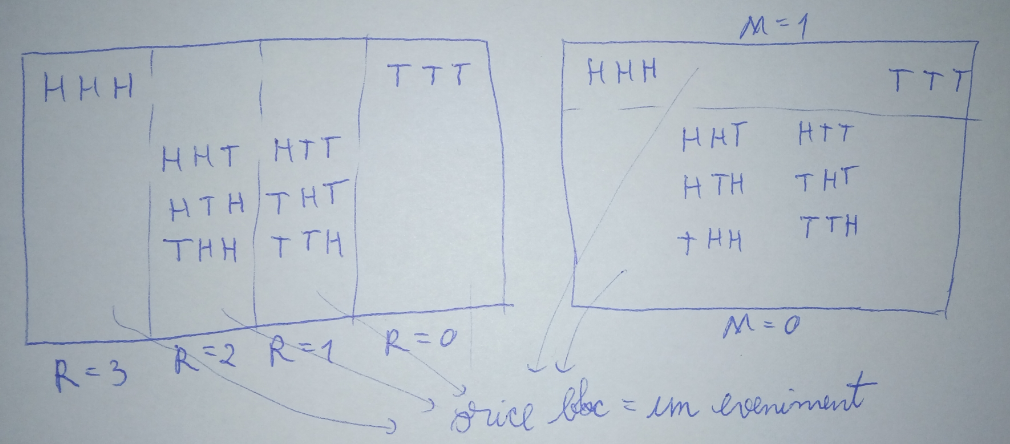
\includegraphics[width=\linewidth]{screenshot007}
	\end{center}
	
	
	"R = 1" va fi o notație pentru un eveniment (deci, o mulțime): "R = 1" = $\{a | R(a) = 1\}$
	
	$P(R = 1) = P(\{a | R(a) = 1\}) = P(\{HTT,THT,TTH\}) \stackrel{\text{adit.num.}}{=} P(\{HTT\}) + P(\{THT\}) + P(\{TTH\}) \stackrel{\text{pp.echiprob.}}{=}\frac{3}{8}$
	
	Calculând P(R = 0), P(R = 1), P(R = 2), P(R = 3), obținem:
	
	$R: \begin{pmatrix}
	0 &1& 2& 3\\
	\frac{1}{8} & \frac{3}{8} & \frac{3}{8} & \frac{1}{8}
	\end{pmatrix}$ - prima linie = valorile posibile ale lui $R$; a doua linie = probabilitățile asociate valorilor
	
	$P(R \in \{0,1\}) = P(R = 0 \cup R = 1) = P(\{a | R(a) = 0\} \cup \{b | R(b) = 1\}) = P(\{TTT\} \cup \{THH, THT, TTH\}) \stackrel{\text{adit.num.}}{=} P(\{TTT\}) + P(\{THH, THT, TTH\}) = P(R = 0) + P(R = 1)$
	
	$P(R = 2|M = 1) = \frac{P(R = 2, M = 1)}{P(M = 1)} = 0$
	
	
	
%	Sunt $R$ și $M$ independente? Nu, pentru că putem observa că $P(R = 2|M=1) = 0 \neq \frac{3}{8} = P(R = 2)$, adică $\exists r = 2 \in \text{Val}(R), m = 1 \in \text{Val}(M)$ astfel încât $P(R = 2 | M = 1) \neq P(R = 2)$.
	
	\textit{Exemplu}:
	
	Dacă $X:\begin{pmatrix}
	-1 & 0 & 1\\
	\frac{1}{2} & \frac{1}{4} & \frac{1}{4}
	\end{pmatrix}$, atunci:
	
	$X^2:\begin{pmatrix}
	0 & 1\\
	P(X^2 = 0) & P(X^2 = 1)
	\end{pmatrix} = 
	\begin{pmatrix}
	0 & 1\\
	P(X = 0) & P(X = -1 \cup X = 1)
	\end{pmatrix}=
	\begin{pmatrix}
	0 & 1\\
	P(X = 0) & P(X = -1) + P(X = 1)
	\end{pmatrix} = \begin{pmatrix}
	0 & 1\\
	\frac{1}{4} & \frac{1}{2} + \frac{1}{4}
	\end{pmatrix}$
	
	și
	
	$2X: \begin{pmatrix}
	-2 & 0 & 2\\
	P(2X = -2)&P(2X=0)&P(2X=2)
	\end{pmatrix} = \begin{pmatrix}
	-2 & 0 & 2\\
	P(X = -1)&P(X=0)&P(X=1)
	\end{pmatrix} =
	\begin{pmatrix}
	-2 & 0 & 2\\
	\frac{1}{2} & \frac{1}{4} & \frac{1}{4}
	\end{pmatrix}$

\textbf{	Regula pentru exemplul de mai sus: aplicați ridicarea la pătrat, înmulțirea cu 2 etc. DOAR valorilor lui $X$, nu și probabilităților!!!}
	
	\textit{Exemplu}:
	
	Dacă $X : \begin{pmatrix}
	0 & 1\\
	\frac{1}{2} & \frac{1}{2}
	\end{pmatrix}$ și $Y : \begin{pmatrix}
	1 & 2\\
	\frac{1}{3} & \frac{2}{3}
	\end{pmatrix}$, atunci:
	
	$X + Y: \begin{pmatrix}
	1 & 2 & 3\\
	\frac{1}{2} \cdot \frac{1}{3} & \cdots & \cdots
	\end{pmatrix}$
	?
	NU!!! În acest caz, nu putem calcula probabilitățile asociate lui $X + Y$, pentru că nu avem destule informații:
	$X + Y: \begin{pmatrix}
	1 & 2 & 3\\
	P(X = 0,Y = 1) & P(X = 0, Y = 2) + P(X = 1, Y = 1) & P(X = 1, Y = 2)
	\end{pmatrix}$.
	
	\textbf{Definiții}: 
	
	\textbf{Funcție masă de probabilitate} (\textit{probability mass function} - \textbf{pmf}) pentru variabila $X$: 
	
	$p : \mathbb{R} \rightarrow [0,1]$, $p(x) = P(X = x)$
	
	\textbf{Funcție cumulativă de distribuție} (\textit{cumulative distribution function} - \textbf{cdf}) pentru variabila $X$:
	
	$F : \mathbb{R} \rightarrow [0,1]$, $F(x) = P(X \leq x)$
	
	\textit{Exemplu}:
	
	Scrieți pmf și cdf pentru
	$X : \begin{pmatrix}
	1 & 2& 3\\
	\frac{1}{4} & \frac{1}{4} & \frac{1}{2}
	\end{pmatrix}$.
	
	pmf:
	
	$p(1) = \frac{1}{4}$
	
	$p(2) = \frac{1}{4}$
	
	$p(3) = \frac{1}{2}$
	
	cdf:
	
	$F(1) = \frac{1}{4}$
	
	$F(2) = \frac{1}{4} + \frac{1}{4} = \frac{1}{2}$
	
	$F(3) = \frac{1}{4} + \frac{1}{4} + \frac{1}{2} = 1$
	
	\textbf{Cum verificăm dacă o funcție este pmf pentru o var. al. X?}
	\begin{itemize}
		\item $p(x) \geq 0, \forall x \in \text{Val}(X)$
		\item $\sum_{x \in \text{Val}(X)}p(x) = 1$
	\end{itemize}
	
\textbf{\large{Medie, varianță, covarianță}}
	
	Există două funcții uzuale care, aplicate unei variabile aleatoare, furnizează câte un număr: \textbf{media}/valoarea așteptată (E = media ponderată a valorilor lui X cu ponderile date de probabilități) și \textbf{varianța} (Var = \textit{depărtarea} la pătrat, în medie, a valorilor lui X față de medie).
	
	\textit{Exemplu}:
	
	Dacă $X : \begin{pmatrix}
	-1 & 0 & 1 & 2\\
	\frac{1}{6} & \frac{1}{6} & \frac{1}{6} & \frac{1}{2}
	\end{pmatrix}$, atunci:
	
	$E[X] = (-1) \cdot \frac{1}{6} + 0 \cdot \frac{1}{6} + 1 \cdot \frac{1}{6} + 2 \cdot \frac{1}{2} = 1$
	
	$X - E[X] = X - 1: \begin{pmatrix}
	-1-1 & 0-1 & 1-1 & 2-1\\
	\frac{1}{6} & \frac{1}{6} & \frac{1}{6} & \frac{1}{2}
	\end{pmatrix}$ = $\begin{pmatrix}
	-2 & -1 & 0 & 1\\
	\frac{1}{6} & \frac{1}{6} & \frac{1}{6} & \frac{1}{2}
	\end{pmatrix}$
	
	$(X - E[X])^2 = (X - 1)^2: \begin{pmatrix}
	0 & 1 & 4\\
	\frac{1}{6} & \frac{1}{6} + \frac{1}{2} & \frac{1}{6}
	\end{pmatrix}$ = $\begin{pmatrix}
	0 & 1 & 4\\
	\frac{1}{6} & \frac{4}{6} & \frac{1}{6}
	\end{pmatrix}$
	
	$E[(X - E[X])^2] = E[(X - 1)^2] = 0 \cdot \frac{1}{6} + 1 \cdot \frac{4}{6} + 4 \cdot \frac{1}{6} = \frac{8}{6} = \frac{4}{3}$
	
	$\Rightarrow \text{Var}(X) = \frac{4}{3}$
	
	\textit{Observație}: media nu trebuie neapărat să fie în intervalul [0,1] și nu trebuie neapărat să aparțină lui Val(X). \textit{Exemplu}:
	
	$X:\begin{pmatrix}
	10&20\\
	\frac{1}{2}&\frac{1}{2}
	\end{pmatrix}$
	
	$E[X] = 10 \cdot \frac{1}{2} + 20 \cdot \frac{1}{2} = 25$
	
	\textit{Observație}: De ce calculăm Var cu \textit{la pătrat}? Pentru că:
	\begin{itemize}
		\item $E[X - E[X]] = 0$
		\item Matematica pentru $E[|X - E[X]|]$ este mai grea decât pentru $E[(X - E[X])^2]$
	\end{itemize}
	
	\textit{Observație}: Din cauza pătratului, unitățile de măsură vor fi la pătrat (dolari$^2$, lei$^2$ etc.). Pentru a reveni la unitatea de măsură inițială, folosim \textbf{deviația standard}:
	$\sqrt{Var(X)}$.
	
	\textit{Observație}: Dacă vă întrebați la ce poate fi bună varianța, un exemplu este următorul. Să zicem că vreți să jucați un joc. Vă dau două jocuri la dispoziție:
	\begin{enumerate}
		\item Arunci o monedă. Dacă iese \textit{heads}, câștigi x dolari, altfel, pierzi x dolari.
		\item Arunci o monedă. Dacă iese \textit{heads}, câștigi y dolari, altfel, pierzi y dolari.
	\end{enumerate}
	Fie X = câștigul (posibil negativ) de la 1
	
	Y = câștigul (posibil negativ) de la 2.
	
	Vă zic că E[X] = E[Y] = 0. Alege jocul SAU întreabă-mă o altă caracteristică pentru X și Y ca să te lămurești. Dacă nu prea-ți pasă, ai să alegi unul din cele două jocuri fără să mă întrebi. Dacă totuși îți pașă, poți să mă întrebi de varianță și îți zic: Var(X) = 1.000.000 și Var(Y) = 1. Acest lucru înseamnă că la primul joc riști mai mult decât la al doilea (la primul caștigi/pierzi mai mult decât la al doilea) pentru că depărtarea față de medie (care este 0 în ambele cazuri) este mai mare în primul caz. Hai să vedem ce stătea în spatele lui X și Y:
	
	$X: \begin{pmatrix}
	-1000 & 1000\\
	\frac{1}{2} & \frac{1}{2}
	\end{pmatrix}$
	
	$Y: \begin{pmatrix}
	-1 & 1\\
	\frac{1}{2} & \frac{1}{2}
	\end{pmatrix}$
	
	Într-adevăr, la primul câștigăm/pierdem mai mult (1000 de dolari)!
	
	

	Media și varianța erau funcții care, aplicate unei variabile aleatoare, furnizau un număr real. Dacă ele erau aplicate unei singure variable aleatoare, \textbf{covarianța} se aplică pe două:
	
	\textbf{Definiție}:
	
	Cov(X,Y) = E[(X - E[X])(Y - E[Y])]
	
	Informație++: o valoare mare pentru covarianță indică faptul că există oarecum o dependență liniară între cele 2 variabile ($X \approx aY + b$).
	
	\textbf{\large{Altele}}
	
	Probabilități:
	\begin{itemize}
		\item \textbf{corelate}: de exemplu, $P(X=1, Y=2)$
		\item \textbf{marginale}: de exemplu, $P(X=1)=\sum_{y\in \text{Val}(Y)}P(X=1,Y=y)$
		
		\textit{Observație}: De ce se cheamă așa? Pentru că, având un tabel cu probabilitățile corelate ale lui X și Y, pentru a afla P(X=x) sau P(Y=y) se calculează suma pe o linie sau o coloană și rezultatul se trece la \textit{marginea} tabelului. \textit{Exemplu} pentru $P(X=0)$:
		
		$P(X = 0) \stackrel{\text{pb.marg.}}{=} P(X = 0,Y = 0) + P(X = 0, Y = 1)$
		
		\begin{center}
			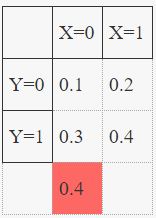
\includegraphics{screenshot006}
		\end{center}
		
		$P(X = 0) = 0.1 + 0.3 = 0.4$
		
		\item \textbf{condiționale}: de exemplu, $P(X=1|Y=2)$
	\end{itemize}

	\textbf{Definiție} (slabă, dar intuitivă):
	$X$, $Y$ - variabile aleatoare \textbf{independente} ($P(Y = y) \neq 0, \forall y \in \text{Val}(Y)$): 
	
	$P(X = x|Y = y) = P(X = x), \forall x \in \text{Val}(X), \forall y \in \text{Val}(Y)$
	
	\textbf{Definiție} (tare):
	$X$, $Y$ - variabile aleatoare \textbf{independente}: 
	
	$P(X = x, Y = y) = P(X = x) P(Y = y), \forall x \in \text{Val}(X), \forall y \in \text{Val}(Y)$
	
	Atenție! La evenimente aleatoare trebuie să verificați doar o singură relație pentru a verifica independența, dar aici, la variabile aleatoare, aveți mai multe relații de verificat (cele din definiție).
	
	Varianta condițională a ultimei definiții:
	$X$, $Y$ - variabile aleatoare \textbf{independente condițional} față de variabila aleatoare $Z$ ($P(Z=z)\neq 0, \forall z\in \text{Val}(Z)$): 
	
	$P(X = x, Y = y|Z=z) = P(X = x|Z=z) P(Y = y|Z=z)$, 
	
	$\forall x \in \text{Val}(X), \forall y \in \text{Val}(Y), \forall z \in \text{Val}(Z)$
	
	\textbf{\large{Formule}}
	
	$$E[aX+bY+c] = aE[X] + bE[Y] + c\text{ - \textbf{liniaritatea mediei}}$$
	
	$$\text{Var}[aX+bY+c] = a^2\text{Var}[X] + b^2\text{Var}[Y] + 2ab\text{Cov}[X,Y]$$
	
	$$\text{Var}[X] = E[X^2] - (E[X])^2$$
	
	$$\text{Cov}[X,Y] = E[XY] - E[X]E[Y]$$
	
	$$X,Y\text{ - independente }\Rightarrow Cov[X,Y]=0$$
	
	$$X,Y\text{ - independente }\centernot\Leftarrow Cov[X,Y]=0$$
	
	$$\text{Cov}[X,Y] = 0 \Rightarrow E[XY] = E[X] E[Y]$$
	
	$$\text{Cov}[X,Y] = 0 \Rightarrow \text{Var}[X+Y] = \text{Var}[X] + \text{Var}[Y]$$
	
	\textbf{\large{Distribuție de probabiitate}}
	
	- se referă la probabilitățile asociate
	\begin{itemize}
		\item fie rezultatelor unui experiment aleator
		\item fie unei variabile aleatoare
	\end{itemize}
	
	- sunt unele care apar în mai multe situații, așa că oamenii le-au analizat și le-au dat nume

	\textit{Exemple}:
	
	\begin{itemize}
		\item distribuția \textbf{uniformă}
		$X : \begin{pmatrix}
		v_1 & v_2 &\dots & v_n\\
		\frac{1}{n} & \frac{1}{n} & \dots & \frac{1}{n}
		\end{pmatrix}$
		
		\textit{Exemplu}: $X : \begin{pmatrix}
		1 & 2&3\\
		\frac{1}{3} & \frac{1}{3} &\frac{1}{3}
		\end{pmatrix}$
		\item distribuția \textbf{Bernoulli}
		
		Experimentul din spate: aruncarea monedei
		
		X = a căzut \textit{heads}? = de căte ori a căzut \textit{heads}? (0 sau 1)
		
		$X:\begin{pmatrix}
		0&1\\
		1-p&p
		\end{pmatrix}$, $p \in [0,1]$
		
		\textit{Exemplu}: $X : \begin{pmatrix}
		0 & 1\\
		0.3 & 0.7
		\end{pmatrix}$
		\item distribuția \textbf{categorială}
		$X : \begin{pmatrix}
		v_1 & v_2 &\dots & v_n\\
		p_1 & p_2 & \dots & p_n = 1-(p_1+\dots+p_{n-1})
		\end{pmatrix}$
		
		\textit{Exemplu}: $X : \begin{pmatrix}
		1 & 2 &3\\
		0.1 & 0.3& 0.6
		\end{pmatrix}$
		
		\item distribuția \textbf{binomială}
		
		Experimentul din spate: n aruncări \textit{independente} ale monedei
		
		X = de câte ori a căzut \textit{heads}?
		
		$X : \begin{pmatrix}
		0 & 1 &\dots&k&\dots&n\\
		C_n^0p^0(1-p)^n & C_n^1p^1(1-p)^{(n-1)}&\dots&C_n^kp^k(1-p)^{(n-k)}&\dots&C_n^np^n(1-p)^0
		\end{pmatrix}$
		
		\textit{Observații}:
		\begin{itemize}
			\item Dacă $n=1$, atunci suntem în cazul distribuției Bernoulli.
			\item X = de câte ori a căzut \textit{heads} = (de câte ori a căzut \textit{heads} la prima aruncare) + (de câte ori a căzut \textit{heads} la a doua aruncare) + $\dots$ + (de câte ori a căzut \textit{heads} la a n-a aruncare), unde fiecare termen este o variabilă aleatoare de tip Bernoulli.
		\end{itemize}
	\end{itemize}
	\newpage
	\textbf{\large{Schemă de final}}
	\begin{enumerate}
		\item Variabile aleatoare
		\begin{enumerate}
			\item definiție
			\item pmf
			\item cdf
			\item operații cu variabile aleatoare ($X^2$, $2X$, $X+Y$ etc.)
			\item E, Var, deviația standard, Cov
			\item probabilități
			\begin{enumerate}
				\item corelate
				\item marginale
				\item condiționale
			\end{enumerate}
			\item\begin{enumerate}
				\item independență
				\item independență condițională
			\end{enumerate}
			\item Formule
		\end{enumerate}
		\item Distribuții de probabilitate
			\begin{enumerate}
				\item uniformă
				\item Bernoulli
				\item categorială
				\item binomială
			\end{enumerate}
	\end{enumerate}
	
\end{document}